\documentclass[a4paper,10pt]{article}

\usepackage{préambule}
\usetikzlibrary{angles,arrows,arrows.meta,calc,intersections,quotes}

\makeatletter
\renewcommand{\maketitle}{%
{\scriptsize colle dans ton cahier d'exercices}
	\begin{center}
		\LARGE
		\myuline{\@title}
		\vspace{0.5em}
	\end{center}
}
\makeatother

\title{Activité : rebonds}
\date{}
\author{}

\begin{document}

\maketitle

On lance une boule de bowling sur une piste, sur laquelle il y a des murs sur le côté sur lesquels la droite rebondit.

\begin{enumerate}
	\item Sur la figure suivante, quelle est la mesure de l'angle $\widehat{ABC}$ ?

	      \begin{minipage}{0.4\textwidth}
		      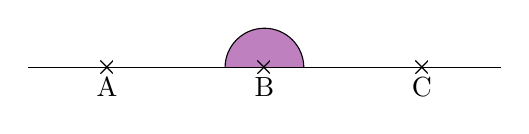
\begin{tikzpicture}
			      \coordinate (A) at (-2,0);
			      \coordinate (B) at (0,0);
			      \coordinate (C) at (2,0);

			      \draw pic[draw,fill=violet!50,angle radius=0.5cm] {angle=C--B--A};

			      \draw (-3,0) -- (3,0);
			      \foreach \p in {A,B,C} {
					      \node at (\p) {×};
					      \node[below] at (\p) {\p};
				      }
		      \end{tikzpicture}
	      \end{minipage} \hspace{1em}
	      \begin{minipage}{0.45\textwidth}
		      $\widehat{ABC} = ..........$
	      \end{minipage}
	\item Lorsque la boule rebondit sur une paroi, sa trajectoire forme l'angle suivant : \vspace{1em}

	      \begin{minipage}{0.35\textwidth}
		      \begin{center}
			      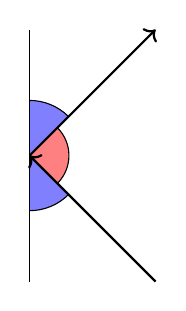
\begin{tikzpicture}[scale=0.8]
				      \coordinate (A) at (0,-2);
				      \coordinate (O) at (0,0);
				      \coordinate (B) at (0,2);
				      \coordinate (X) at (2,-2);
				      \coordinate (Y) at (2,2);

				      \draw pic[draw,fill=blue!50,angle radius=0.7cm] {angle=Y--O--B};
				      \draw pic[draw,fill=red!50,angle radius=0.5cm] {angle=X--O--Y};
				      \draw pic[draw,fill=blue!50,angle radius=0.7cm] {angle=A--O--X};

				      \draw (A) -- (B);
				      \draw[thick,->] (X) -- (O);
				      \draw[thick,->] (O) -- (Y);
			      \end{tikzpicture}
		      \end{center}
	      \end{minipage} \hspace{1em}
	      \begin{minipage}{0.5\textwidth}
		      Où les deux angles bleus ont la même mesure. \vspace{2em}

		      Si un angle bleu mesure 45°, combien mesure l'angle rouge ? ..........
	      \end{minipage}
	\item Reproduit la figure ci-dessous dans ton cahier : \vspace{1em}

	      \begin{minipage}{0.35\textwidth}
		      \begin{center}
			      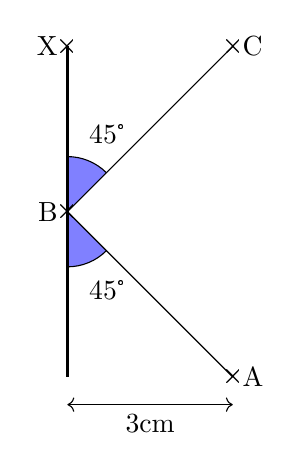
\begin{tikzpicture}[scale=0.7]
				      \coordinate (A) at (0,0);
				      \coordinate (B) at (-3,3);
				      \coordinate (C) at (0,6);
				      \coordinate (X) at (-3,6);
				      \coordinate (Y) at (-3,0);

				      \draw pic[draw,fill=blue!50,angle radius=0.7cm,"45°" shift={(0.35cm,-0.6cm)}] {angle=Y--B--A};
				      \draw pic[draw,fill=blue!50,angle radius=0.7cm,"45°" shift={(0.35cm,0.6cm)}] {angle=C--B--X};

				      \draw (A) -- (B) -- (C);
				      \draw[thick] (X) -- (Y);

				      \coordinate (A1) at ($(A) + (0,-0.5)$);
				      \coordinate (Y1) at ($(Y) + (0,-0.5)$);
				      \draw[<->] (A1) -- node[below] {3cm} (Y1);

				      \foreach \p/\pos in {A/right,B/left,C/right,X/left} {
						      \node at (\p) {×};
						      \node[\pos] at (\p) {\p};
					      }
			      \end{tikzpicture}
		      \end{center}
	      \end{minipage} \hspace{1em}
	      \begin{minipage}{0.45\textwidth}
		      La distance AC est ........... \vspace{1em}

		      La distance XC est ...........
	      \end{minipage}
	\item On fait à présent deux rebonds :
	      \vspace{1em}

	      \begin{minipage}{0.35\textwidth}
		      \begin{center}
			      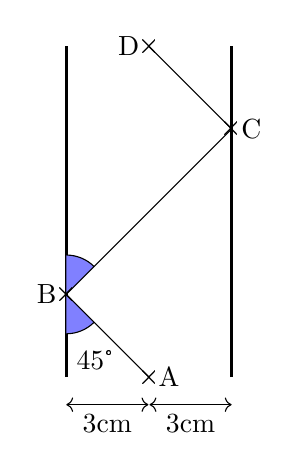
\begin{tikzpicture}[scale=0.35]
				      \coordinate (X) at (-3,0);
				      \coordinate (Y) at (-3,12);
				      \draw[very thick] (X) -- (Y);
				      \draw[very thick] (3,0) -- (3,12);

				      \coordinate (A) at (0,0);
				      \coordinate (B) at (-3,3);
				      \coordinate (C) at (3,9);
				      \coordinate (D) at (0,12);

				      \draw pic[draw,fill=blue!50,angle radius=0.5cm] {angle=C--B--Y};
				      \draw pic[draw,fill=blue!50,angle radius=0.5cm,"45°" shift={(0.25cm,-0.55cm)}] {angle=X--B--A};
				      \draw (A) -- (B) -- (C) -- (D);

				      \foreach \p/\pos in {A/right,B/left,C/right,D/left} {
						      \node at (\p) {×};
						      \node[\pos] at (\p) {\p};
					      }

				      \draw[<->] (-3,-1) -- node[below] {3cm} ($(A) + (-0.02,-1)$);
				      \draw[<->] ($(A) + (0.02,-1)$) -- node[below] {3cm} (3,-1);
			      \end{tikzpicture}
		      \end{center}
	      \end{minipage} \hspace{1em}
	      \begin{minipage}{0.5\textwidth}
		      La mesure de l'angle $\widehat{BCD}$ est .......... \vspace{1em}

		      La distance AD est ..........
	      \end{minipage}
	\item La piste de bowling a la forme suivante : \vspace{0.5em}

	      \begin{minipage}{0.4\textwidth}
		      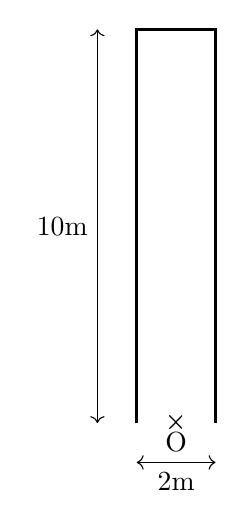
\begin{tikzpicture}[scale=0.5]
			      \draw[very thick] (-1,0) -- ++(0,10) -- ++(2,0) -- ++(0,-10);
			      \draw[<->] (-2,0) -- node[left] {10m} ++(0,10);
			      \draw[<->] (-1,-1) -- node[below] {2m} (1,-1);

			      \node (O) at (0,0) {×};
			      \node[below] at (O) {O};
			      %   \draw (0,0) -- (-1,1) -- (1,3) -- (-1,5) -- (1,7) -- (-1,9) -- (0,10);
		      \end{tikzpicture}
	      \end{minipage} \hspace{1em}
	      \begin{minipage}{0.5\textwidth}
		      Reproduit cette figure dans ton cahier, en prenant 1m ⇒ 1cm.

		      On lance une boule depuis le point O, avec un angle de 45° vers la gauche.

		      Trace la trajectoire de la boule le long de la piste, et marque le point d'arrivée à l'autre bout.
	      \end{minipage}
\end{enumerate}

\end{document}